\section{\red{Modelling data}}\label{sec:implementation}
\subsection{GM linearization}
To find coefficients for the linearization of GM, we generate a number of cargo and ballast water distributions, which determines the lcg and vcg of the vassel. From these values, we can look up values of the draft, trim, and the GM of the vessel. %lcg is calculated, draft, trim and m are looked up in table given displacement and lcg. vcg is ``calculated'' from an assumption of where the vcg is. gm = m - vcg.
We then make a multidimensional regression to determine the (best) linear function for the GM as a function of the values for the weight on deck, the weight below deck, the weight of ballast water, the draft and the trim. The GM of each of the cargo and ballast distributions plotted against the GM given by the resulting function is shown in Figure~\ref{fig:predictGM}. If the prediction were precise, all these points would lie on the diagonal line. The $R^2$ value is $0.977$, and as can also be seen from the figure, the GM prediction is very reasonable.

\begin{figure}
	\centering
		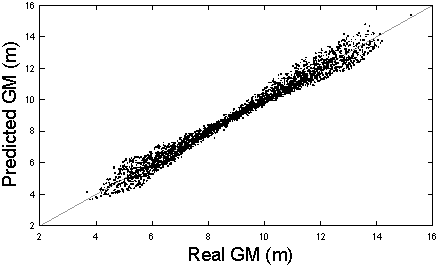
\includegraphics[scale=0.35]{figures/gnuPlotAll.pdf}
	\caption{Prediction of GM from linear function}
	\label{fig:predictGM}
\end{figure}

%\subsubsection{Generation of data}
The cargo and ballast water distributions are generated by looping through combinations of intervals of percentage TEU-usage above and below deck in each bay, plus amount of ballast water. For each bay above and below deck, an amount of containers (in TEU) is randomly chosen in the given intervals, and 0-15\% above deck and 0-25\% below deck of these are chosen to be 20' containers. A weight of these containers are then chosen from a distribution depending on whether it is on or below deck as given below.

\begin{center}
\begin{tabular}{l|rr}
		&	Above deck &	Below deck\\ 
		\hline
25t	&		10-15\%	 &	20-25\%	\\	
15t	&		25-35\%	 &	35-40\% \\
5t	&	remainder  &	remainder\\
\end{tabular}
\end{center}

From these cargo distributions we then calculate the lcg and vcg. The lcg is straighforward since we know the placement of cargo in bays. For the vcg, we assume that the containers on deck have been stacked with the heaviest containers in the bottom of the stacks with lighter containers above. Below deck, the shape of the hull can be seen as either triangular or as box-shaped. Containers can be stowed more freely, and we have decided to assume a vcg corresponding to the middle of the stack (for box-shaped bays) and 2/3 up for triangular-shaped boxes. %\red{[Egentlig kunne vi vel bare have bestemt (tilfældigt) hvordan tingene skulle stå og så beregne den korrekte vcg istedet for at approximere den ved at sige at "vcg nok ligger i midten under dæk"]}.  

We only use cargo and ballast distributions that makes the vessel have at least 55\% of its maximal displacement. 

%\subsubsection{\red{Discussion}}
\red{Why it is reasonable to not have more points with low GM. I can't remember what we discussed.}

%%%%%%%%%%%%%%%%%%%%%%%%%%%%%%%%%%%%%%%%%%%%%%%%%%%%%%%%%%%%%%
\subsection{Polygon for allowable lashing-configurations} 
In our model, allowable combinations of containers of each length+height are described by a polygon whose corners are given by the maximal numbers of containers of each combination of length+height at two values for GM.  

%\subsubsection{Obtaining data}
For a low but realistic GM value (higher than $L^{\ttt{gm}-}$) we have loaded a representative bay over deck with as many 20' containers of one weight class as possible until the lashing constraints were violated according to the loading computer. The same were then done for a GM value equal to $L^{\ttt{gm}+}$. The maximal number of 20' containers possible to load at a GM value of $L^{\ttt{gm}-}$ where then extrapolated from these two value. 
Then the process were repeated for all other combinations of length+weight-classes.
When doing so, when the limit was first reached, we added a horizontal ``layer'' of lighter containers (with a weight that was as high as possible within the lashing constraints) and translated this weight back to a number of containers of the considered weight class. This number were then added to the previous found number of containers and made up the limit.
% Har gjort det for GM = 3 og GM = 15. Minimal value for GM er dog sat til 0, men der har vi ekstrapoleret disse linier til. Så får vi ikke skåret for meget af nede omkring meget lave GM

%\subsubsection{\red{Discussion}} 
\red{Why is this reasonable? Unlike our other estimations, this is not a precautionary measure/conservative estimate.}

\section{Implementation}
%\paragraph{Horizon}
In the implementation, instead of having container groups with a deadline later than the last date in the network, all container groups have a deadline in $\mc{D}$, i.e. $\mc{G} = \mc{G}'$. Instead we use a \emph{horizon}, which is a date in $\mc{D}$ after which new cargo is not exported, and we only gain revenue for the containers delivered before the horizon. 
The port calls between the relevant deadline %=45
and the last date, only serve to ``empty'' the vessel.
So $Ex^{g-}_e = Ex^{g+}_e = 0$ for edges $(I^\ttt{x},i)$ to a node $i$ after the horizon, and \eqref{obj} only sum over the nodes within the horizon. 
Likewise, the standard capacity for vessels \eqref{sailingCon} only apply fully to edges within the horizon (since some of the constraints will not hold for half-empty vessels that are artificially created. So after the horizon, only the vessel capacity constraints \eqref{cap20}-\eqref{capDisp} of the vessel-constraints are enforced. % Also overstowage is enforced after deadline, but not the crane moves constraints
\\\\
%\paragraph{Variable domains}
In the model presented in Section~\ref{sec:model}, many variables are a priori known to be zero. For example, container groups with a deadline $d\in\mc{D}$ have to be delivered before $d$, and therefore the containers cannot flow on an edge $(i,j)\in\mc{E}^\ttt{v}$ where the day $d'$ corresponding to the node $j$ is greater than $d$. We do not define and use these variables (and similar ones) in the constraints.
\\\\
Do to availability of data, all vessels are assumed to be of the same type/build, i.e. their basic data is the same.
\\\\
Several vessels might arrive at the same port at the same day; this is modeled in such a way that the vessels are ordered and the one which comes first in this order also comes first at the port call. 
